\section{Auswertung}
\label{sec:Auswertung}

%\begin{figure}
%  \centering
%  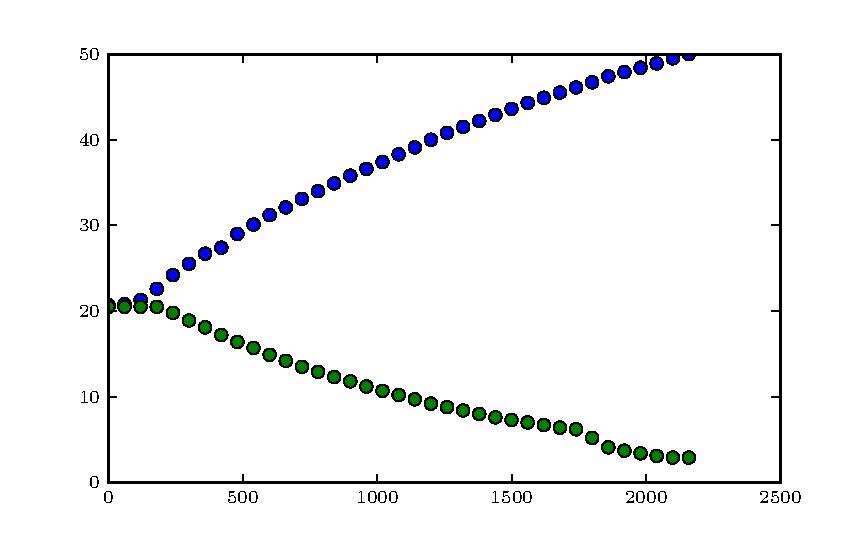
\includegraphics{plot.pdf}
%  \caption{Plot.}
%  \label{fig:plot}
%\end{figure}




%%%%%%%%%%%%%%%%%%%%%%%%%%%%%%%%%%%%%%
%Strömungsprofil
%%%%%%%Pumpleistung 70%
Zur Untersuchung der Streuintensität und der Momentangeschwindigkeit in Abhängigkeit zur Eindringtiefe ist es zunächst notwendig, die Eindringtiefe $x_{\mathrm{sec}}$ welche in der Messung in Microsekunden aufgenommen wurde, in die Eindringtiefe $x_{\mathrm{mm}}$ in Millimetern umzurechnen.
Es werden hierzu zunächst die Verhältnisse zwischen $x_{\mathrm{sec}}$ und $x_{\mathrm{mm}}$ für beide Materialien bestimmt.\\
Hierbei ist die Vorlaufstrecke, welche sich aus der Vorlaufstrecke im Prisma und der Wand der untersuchten Röhre ergibt, als $x_\mathrm{vor}=\SI{33.2}{\milli\meter}$ ebenso bekannt, wie die Schallgeschwindingkeit im Prisma $c_\mathrm{P}=\SI{2700}{\meter\per\second}$, in der Dopplerphantomflüssigkeit $c_\mathrm{L}=\SI{1800}{\meter\per\second}$ sowie der Innendurchmesser der verwendeten Strömungsröhre $d_\mathrm{innen}=\SI{10}{\milli\meter}$ nach Versuchsanleitung \cite{Anleitung}.\\
Da nicht bekannt ist, wie groß die Schallgeschwindigkeit im Röhrenmaterial ist, wurde für diese dieselbe Schallgeschwindigkeit wie im Prisma angenommen.
Die Zeit, welche der Ultraschall benötigt, um die Vorlaufstrecke zu durchlaufen, ergibt sich nach
\begin{equation*}
  t=\frac{s}{v} \text{,}
\end{equation*}
mit $s$ als Vorlaufstrecke und $v=c_\mathrm{P}$ zu:
\begin{equation*}
    t_\mathrm{vor}\approx\SI{12.29}{\second}\text{.}
\end{equation*}
Das Verhältnis zwischen Eindringtiefe in Mikrosekunden und Eindringtiefe in Millimetern ist daher $\frac{x_\mathrm{sec}}{x_\mathrm{mm}}=\SI{0.37}{\micro\second\per\milli\meter}$ im Prisma. Vollkommen analog ergibt sich selbiges Verhältnis in der Dopplerphantomflüssigkeit zu $\frac{x_\mathrm{sec}}{x_\mathrm{mm}}=\SI{0.556}{\micro\second\per\milli\meter}$.
\\Somit kann die gemessene Eindrigtiefe $x_\mathrm{sec}$ in $x_\mathrm{mm}$ umgerechnet werden. Die Ergebnisse finden sich in Tabelle \ref{tab:pl70} für die Messung bei einer Pumpleistung von $P=\SI{70}{\percent}$ sowie in Tabelle  \ref{tab:pl45} für $P=\SI{45.2}{\percent}$.
Zudem sind dort die zugehörigen Streuintensitätswerte $I_\mathrm{S}$ sowie die Dopplerverschiebungen $\Delta \nu$ und die hieraus nach Formel \eqref{eqn:verschiebung} berechneten Momentangeschwindigkeiten $v_\mathrm{mom}$ eingetragen.

\begin{figure}
  \centering
  \includegraphics{Bilder/I45-2.pdf}
  \caption{Streuintensität $I_\mathrm{S}$ aufgetragen gegen die Eindringtiefe $x_\mathrm{mm}$ bei einer Pumpleistung von $\SI{45.2}{\percent}$. }
  \label{fig:I45}
\end{figure}
\begin{figure}
  \centering
  \includegraphics{Bilder/I70.pdf}
  \caption{Streuintensität $I_\mathrm{S}$ aufgetragen gegen die Eindringtiefe $x_\mathrm{mm}$ bei einer Pumpleistung von $\SI{70}{\percent}$. }
  \label{fig:I70}
\end{figure}

\begin{table}
  \centering
  \caption{Messdaten zur Berechnung des Strömungsprofil bei einer Pumpleistung von $\SI{45.2}{\percent}$.}
  \label{tab:pl45}
  \begin{tabular}{ccccc}
    \toprule
    $x_\mathrm{sec}$/$\si{\micro\second}$ & $x_\mathrm{mm}$/$\si{\milli\meter}$ & $I_\mathrm{S}$/$\si{\square\volt\per\second}$ & $\Delta \nu$/$\si{\Hz}$&$v_\mathrm{mom}$/$\si{\meter\per\second}$ \\
    \midrule
    13,0 & 34,5 & 90,0 & 220,0 & 0,574 \\
    13,5 & 35,4 & 120,0 & 232,0 & 0,605 \\
    14,0 & 36,3 & 155,0 & 269,0 & 0,702 \\
    14,5 & 37,2 & 170,0 & 305,0 & 0,795 \\
    15,0 & 38,1 & 180,0 & 317,0 & 0,827 \\
    15,5 & 39,0 & 208,0 & 305,0 & 0,795 \\
    16,0 & 39,9 & 230,0 & 281,0 & 0,733 \\
    16,5 & 40,8 & 203,0 & 269,0 & 0,702 \\
    17,0 & 41,7 & 196,0 & 232,0 & 0,605 \\
    17,5 & 42,6 & 191,0 & 226,0 & 0,589 \\
    18,0 & 43,4 & 232,0 & 244,0 & 0,636 \\
    18,5 & 44,3 & 444,0 & 256,0 & 0,668 \\
    19,0 & 45,2 & 360,0 & 244,0 & 0,636 \\
    19,5 & 46,1 & 300,0 & 256,0 & 0,668 \\
    \bottomrule
  \end{tabular}
\end{table}
\begin{table}
\centering
\caption{Messdaten zur Berechnung des Strömungsprofil bei einer Pumpleistung von $\SI{70}{\percent}$.}
\label{tab:pl70}
\begin{tabular}{ccccc}
  \toprule
  $x_\mathrm{sec}$/$\si{\micro\second}$ & $x_\mathrm{mm}$/$\si{\milli\meter}$ & $I_\mathrm{S}$/$\si{\square\volt\per\second}$ & $\Delta \nu$/$\si{\Hz}$&$v_\mathrm{mom}$/$\si{\meter\per\second}$ \\
\midrule
13,0 & 34,5 & 90,0 & 439,0 & 1,145 \\
13,5 & 35,4 & 114,0 & 490,0 & 1,278 \\
14,0 & 36,3 & 126,0 & 562,0 & 1,466 \\
14,5 & 37,2 & 140,0 & 623,0 & 1,625 \\
15,0 & 38,1 & 156,0 & 647,0 & 1,687 \\
15,5 & 39,0 & 160,0 & 623,0 & 1,625 \\
16,0 & 39,9 & 176,0 & 574,0 & 1,497 \\
16,5 & 40,8 & 187,0 & 500,0 & 1,304 \\
17,0 & 41,7 & 183,0 & 439,0 & 1,145 \\
17,5 & 42,6 & 206,0 & 421,0 & 1,098 \\
18,0 & 43,4 & 250,0 & 500,0 & 1,304 \\
18,5 & 44,3 & 495,0 & 500,0 & 1,304 \\
19,0 & 45,2 & 438,0 & 500,0 & 1,304 \\
19,5 & 46,1 & 348,0 & 500,0 & 1,304 \\
\bottomrule
\end{tabular}
\end{table}



\begin{figure}
  \centering
  \includegraphics{Bilder/f70.pdf}
  \caption{Strömungsprofil der Dopplerflüssigkeit bei einer Pumpleistung von $\SI{70}{\percent}$.}
  \label{fig:f70}
\end{figure}
\begin{figure}
  \centering
  \includegraphics{Bilder/f45-2.pdf}
  \caption{Strömungsprofil der Dopplerflüssigkeit bei einer Pumpleistung von $\SI{45.2}{\percent}$.}
  \label{fig:f45}
\end{figure}

In Abbildung \ref{fig:I45} und Abbildung \ref{fig:I70} sind die gemessenen Streuintensitäten $I_\mathrm{S}$ gegen die berechnete Momentangeschwindigkeit $v_\mathrm{mom}$ aufgetragen. Für beide Pumpleistungen zeigt sich etwa das erwartete Bild.
Der relativ gleichmäßige Anstieg der Streuintensität für eine Eindringtiefe bis etwa $x_\mathrm{mm}=\SI{43}{\milli\meter}$ ist hierbei verursacht durch die Reflektion an der Dopplerflüssigkeit innerhalb der Röhre. Mit steigender Eindringtiefe steigt daher auch die Intensität der reflektierten Streuintensität $I_\mathrm{S}$ aufgrund der steigenden Zahl an stattfindenden Reflektionen und Streuungen an den Molekülen der Dopplerflüssigkeit mit größer werdender Eindringtiefe.
Der große Anstieg der Streuintensität bei etwas über $x_\mathrm{mm}=\SI{43}{\milli\meter}$ entsteht durch die große Reflektion der einlaufenden Ultraschallwelle an der Wand der Strömungsröhre. Diese wird verursacht durch den größeren Brechungskoeffizienten der Wand der Strömungsröhre gegenüber dem der Dopplerflüssigkeit.


In Abbildung \ref{fig:f45} und Abbildung \ref{fig:f70} sind die gemessenen Momentangeschwindigkeiten gegen die Eindringtiefe aufgetragen. Es zeigt sich ebenso für beide Pumpleistungen etwa das erwartete Bild.
In der Mitte des Strömungsrohrs bei etwas  über $x_\mathrm{mm}=\SI{38}{\milli\meter}$ zeigt sich ein Maximum in der Strömungsgeschwindigkeit.\\
Allgemein zeigt sich ein parabelförmiger Verlauf der Momentangeschwindigkeit mit einem Maximum in der Mitte der Strömungsröhre. Dieser Verlauf ist typisch für laminare Strömungen.
\\Die Strömungsgeschwindigkeit ist hierbei am Rand des Strömungsrohres deutlich geringer als in der Mitte, da zwischen der Wand des Rohres und der Dopplerflüssigkeit stärkere Reibungseffekte auftreten als innerhalb der Dopplerflüssigkeit. Auf ein Molekül der Dopplerflüssigkeit in der Mitte des Strömungsrohrs wirkt eine geringere Bremskraft aufgrund von Reibung als auf ein Molekül am Rand, somit prägt sich mittig des Strömungsrohres eine größere Strömungsgeschwindigkeit als am Rand aus.
